\documentclass[11pt,a4paper]{book}
\usepackage[spanish,es-nodecimaldot]{babel}	% Utilizar español
\usepackage[utf8]{inputenc}					% Caracteres UTF-8
\usepackage{graphicx}						% Imagenes
\usepackage[hidelinks]{hyperref}			% Poner enlaces sin marcarlos en rojo
\usepackage{fancyhdr}						% Modificar encabezados y pies de pagina
\usepackage{float}							% Insertar figuras
\usepackage[textwidth=390pt]{geometry}		% Anchura de la pagina
\usepackage[nottoc]{tocbibind}				% Referencias (no incluir num pagina indice en Indice)
\usepackage{enumitem}						% Permitir enumerate con distintos simbolos
\usepackage[T1]{fontenc}					% Usar textsc en sections
\usepackage{amsmath}						% Símbolos matemáticos

\usepackage{emptypage}
\usepackage[Sonny]{fncychap}                % Capitulos chulos

\usepackage[
    backend=biber,
    style=alphabetic,
    sorting=ynt
]{biblatex}                       % Gestion de bibliografia
\addbibresource{bibliography.bib}

% Comando para poner el nombre de la asignatura
\newcommand{\asignatura}{Trabajo Fin de Grado}
\newcommand{\autor}{Vladislav Nikolov Vasilev}
\newcommand{\titulo}{Implementación de una arquitectura reactiva y deliberativa usando planificación en el entorno de juegos GVGAI}
\newcommand{\subtitulo}{Subtitulo}
\newcommand{\director}{Juan Fernández Olivares}

% Configuracion de encabezados y pies de pagina
\pagestyle{fancy}

% Paginas pares: poner solo el nombre del capitulo
\fancyhead[RE]{}
\fancyhead[LE]{\textbf{\nouppercase{\leftmark}}}

% Paginas impares: poner la seccion y el autor
\fancyhead[LO]{\autor{}}
\fancyhead[RO]{\textbf{\nouppercase{\rightmark}}}

\fancyfoot[L]{Grado en Ingeniería Informática}
\fancyfoot[C]{}
\fancyfoot[R]{\thepage}

% Poner las lineas
\renewcommand{\headrulewidth}{0.4pt}		% Linea cabeza de pagina
\renewcommand{\footrulewidth}{0.4pt}		% Linea pie de pagina

\begin{document}
\pagenumbering{gobble}

% Insertar portada
%%%%%%%%%%%%%%%%%%%%%%%%%%%%%%%%%%%%%%%%%%%%%%%%%%%%%%%%%%%%%%%%%%%%%%%%%%%%%%%%
%                           Portada del proyecto                               %
%%%%%%%%%%%%%%%%%%%%%%%%%%%%%%%%%%%%%%%%%%%%%%%%%%%%%%%%%%%%%%%%%%%%%%%%%%%%%%%%
\begin{titlepage}

\begin{minipage}{\textwidth}

\centering

%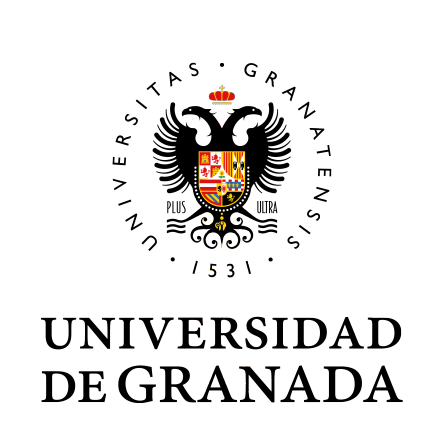
\includegraphics[scale=0.5]{img/ugr.png}\\

\includegraphics[scale=0.3]{img/logo_ugr.jpg}\\[1cm]

\textsc{\Large \asignatura{}\\[0.2cm]}
\textsc{GRADO EN INGENIERÍA INFORMÁTICA}\\[1cm]

\noindent\rule[-1ex]{\textwidth}{1pt}\\[1.5ex]
\textsc{{\Huge \titulo\\[0.5ex]}}
\textsc{{\Large \subtitulo\\}}
\noindent\rule[-1ex]{\textwidth}{2pt}\\[3.5ex]

\end{minipage}

%\vspace{0.5cm}
\vspace{0.7cm}

\begin{minipage}{\textwidth}

\centering

\textbf{Autor}\\ {\autor{}}\\[2.5ex]
\textbf{Rama}\\ {\rama}\\[2.5ex]
\vspace{0.3cm}


\includegraphics[scale=0.3]{img/etsiit.jpeg}

\vspace{0.7cm}
\textsc{Escuela Técnica Superior de Ingenierías Informática y de Telecomunicación}\\
\vspace{1cm}
\textsc{Curso 2019-2020}
\end{minipage}
\end{titlepage}

% Insertar prefacio
%\thispagestyle{empty}
%\cleardoublepage

%\thispagestyle{empty}


\cleardoublepage
\thispagestyle{empty}

%%%%%%%%%%%%%%%%%%%%%%%%%%%%%%%%%%%%%%%%%%%%%%%%%%%%%%%%%%%%%%%%%%%%%%%%%%%
% Resumen en español

\begin{center}
%{\large\bfseries Título del Proyecto: Subtítulo del proyecto}\\
{\large\bfseries \titulo}\\
\end{center}
\begin{center}
\autor\\
\end{center}

%\vspace{0.7cm}
\noindent{\textbf{Palabras clave}: Inteligencia Artificial, Planificación automática, Videojuegos}\\

\vspace{0.7cm}
\noindent{\textbf{Resumen}}\\

A pesar de que la planificación automática ha sido integrada con éxito en muchas aplicaciones
reales, los videojuegos siguen suponiéndole un gran reto debido a lo dinámicos y complejos que son.
Esto ha llevado a que muchos autores hayan intentado integrar arquitecturas deliberativas basadas en
planificación en videojuegos. Sin embargo, las arquitecturas propuestas se centran solamente en un único juego.
Por tanto, en este trabajo presentamos una novedosa arquitectura semiautomática que combina una componente
reactiva con una componente deliberativa basada en planificación en el entorno de juegos GVGAI.
Esta arquitectura está diseñada de manera que permita resolver múltiples juegos del entorno.
Se reciben como entrada un dominio de planificación PDDL y un archivo de configuración YAML que contiene la
correspondencia entre elementos del juego y los predicados PDDL definidos en el dominio y un conjunto de objetivos a
alcanzar. A partir del fichero de configuración, el sistema genera automáticamente problemas PDDL. Utilizando
un planificador en la nube que recibe el dominio PDDL y el problema generado, se obtienen planes para alcanzar
los objetivos propuestos. La ejecución del plan es monitorizada por la componente reactiva, comprobando la existencia
de discrepancias en dicho plan.

\cleardoublepage


\thispagestyle{empty}

%%%%%%%%%%%%%%%%%%%%%%%%%%%%%%%%%%%%%%%%%%%%%%%%%%%%%%%%%%%%%%%%%%%%%%%%%%%
% Abstract en ingles 

\begin{center}
%{\large\bfseries Project Title: Project Subtitle}\\
{\large\bfseries \tituloingles}\\
\end{center}
\begin{center}
\autor\\
\end{center}

%\vspace{0.7cm}
\noindent{\textbf{Keywords}: Artificial Intelligence, Automated Planning, Video Games}\\

\vspace{0.7cm}
\noindent{\textbf{Abstract}}\\

Despite the fact that automated planning has been successfully integrated into many real-world
applications, video games are still considered to be very challenging due to their dynamism
and complexity. This has led many authors to try to integrate planning-based deliberative architectures
into video games. However, the proposed architectures focus only on a single game. Therefore, in this
work we present a novel semi-automatic architecture that combines a reactive component with a
planning-based deliberative component in the GVGAI game environment. This architecture has been designed
so that many of the environment's games can be solved. It receives a PDDL planning domain and a YAML
configuration file that contains both the correspondence between the game's elements and PDDL predicates defined
in the domain and a set of goals to be reached. The system automatically generates PDDL problem files thanks
to the configuration file. By using a planner in the cloud that receives the PDDL domain and the
generated problem, the system obtains plans that allow it to reach the proposed goals. The plan's execution
is monitored by the reactive component, checking the existence of discrepancies in that plan.

\cleardoublepage
\thispagestyle{empty}

\noindent\rule[-1ex]{\textwidth}{2pt}\\[4.5ex]

Yo, \textbf{\autor}, alumno de la titulación Ingeniería Informática de la \textbf{Escuela Técnica Superior
de Ingenierías Informática y de Telecomunicación de la Universidad de Granada}, con NIE X8743846M, autorizo la
ubicación de la siguiente copia de mi Trabajo Fin de Grado en la biblioteca del centro para que pueda ser
consultada por las personas que lo deseen.

\vspace{6cm}

\noindent Fdo: \autor

\vspace{2cm}

\begin{flushright}
Granada a 6 de julio de 2020.
\end{flushright}


\cleardoublepage
\thispagestyle{empty}

\noindent\rule[-1ex]{\textwidth}{2pt}\\[4.5ex]

D. \textbf{\director}, Profesor del Departamento de Ciencias de la Computación e Inteligencia Artificial
de la Universidad de Granada.


\vspace{0.5cm}

\textbf{Informa:}

\vspace{0.5cm}

Que el presente trabajo, titulado \textit{\textbf{\titulo}},
ha sido realizado bajo su supervisión por \textbf{\autor}, y autorizo la defensa de dicho trabajo ante el tribunal
que corresponda.

\vspace{0.5cm}

Y para que conste, expide y firma el presente informe en Granada a 6 de julio de 2020.

\vspace{1cm}

\textbf{El director:}

\vspace{5cm}

\noindent \textbf{\director{} }

\chapter*{Agradecimientos}
\thispagestyle{empty}

       \vspace{1cm}


Quiero empezar dándole las gracias a Ignacio Vellido Expósito por la creación del dominio
simplificado del juego \textit{Boulderdash}. También quiero darle las gracias a mi tutor,
el Dr. Juan Fernández Olivares por darme la oportunidad de trabajar en un proyecto de este tipo.
Y por último, pero no por ello menos importante, quiero darles las gracias a mis padres y a todos
mis amigos, los cuales me han dado todo el apoyo necesario para continuar adelante, incluso
en los momentos más duros.


% Indice
\thispagestyle{empty}
\tableofcontents

% Lista de figuras
\thispagestyle{empty}
\listoffigures

\newpage

% Comenzar la numeracion de las paginas a partir del primer capitulo
\pagenumbering{arabic}
\setlength{\parskip}{1em}

% Insertar capitulo 1: Introduccion
%%%%%%%%%%%%%%%%%%%%%%%%%%%%%%%%%%%%%%%%%%%%%%%%%%%%%%%%%%%%%%%%%%%%%%%%%%%%%%%%
%                    Capitulo 1: Introduccion                                  %
%%%%%%%%%%%%%%%%%%%%%%%%%%%%%%%%%%%%%%%%%%%%%%%%%%%%%%%%%%%%%%%%%%%%%%%%%%%%%%%%

\chapter{Introducción}



%%%%%%%%%%%%%%%%%%%%%%%%%%%%%%%%%%%%%%%%%%%%%%%%%%%%%%%%%%%%%%%%%%%%%%%%%%%%%%%%
%                    Capitulo 2: Antecedentes                                  %
%%%%%%%%%%%%%%%%%%%%%%%%%%%%%%%%%%%%%%%%%%%%%%%%%%%%%%%%%%%%%%%%%%%%%%%%%%%%%%%%

\chapter{Antecedentes}


%%%%%%%%%%%%%%%%%%%%%%%%%%%%%%%%%%%%%%%%%%%%%%%%%%%%%%%%%%%%%%%%%%%%%%%%%%%%%%%%
%                    Capitulo 3: Plan de trabajo                               %
%%%%%%%%%%%%%%%%%%%%%%%%%%%%%%%%%%%%%%%%%%%%%%%%%%%%%%%%%%%%%%%%%%%%%%%%%%%%%%%%

\chapter{Plan de trabajo}


%%%%%%%%%%%%%%%%%%%%%%%%%%%%%%%%%%%%%%%%%%%%%%%%%%%%%%%%%%%%%%%%%%%%%%%%%%%%%%%%
%              Capitulo 4: Arquitectura general del sistema                    %
%%%%%%%%%%%%%%%%%%%%%%%%%%%%%%%%%%%%%%%%%%%%%%%%%%%%%%%%%%%%%%%%%%%%%%%%%%%%%%%%

\chapter{Arquitectura general del sistema}


%%%%%%%%%%%%%%%%%%%%%%%%%%%%%%%%%%%%%%%%%%%%%%%%%%%%%%%%%%%%%%%%%%%%%%%%%%%%%%%%
%                    Capitulo 5: Descripcion detallada                         %
%%%%%%%%%%%%%%%%%%%%%%%%%%%%%%%%%%%%%%%%%%%%%%%%%%%%%%%%%%%%%%%%%%%%%%%%%%%%%%%%

\chapter{Descripción detallada}


%%%%%%%%%%%%%%%%%%%%%%%%%%%%%%%%%%%%%%%%%%%%%%%%%%%%%%%%%%%%%%%%%%%%%%%%%%%%%%%%
%                Capitulo 6: Documentacion de diseño software                  %
%%%%%%%%%%%%%%%%%%%%%%%%%%%%%%%%%%%%%%%%%%%%%%%%%%%%%%%%%%%%%%%%%%%%%%%%%%%%%%%%

\chapter{Documentación de diseño software}


%%%%%%%%%%%%%%%%%%%%%%%%%%%%%%%%%%%%%%%%%%%%%%%%%%%%%%%%%%%%%%%%%%%%%%%%%%%%%%%%
%                    Capitulo 7: Experimentacion                               %
%%%%%%%%%%%%%%%%%%%%%%%%%%%%%%%%%%%%%%%%%%%%%%%%%%%%%%%%%%%%%%%%%%%%%%%%%%%%%%%%

\chapter{Experimentación}


%%%%%%%%%%%%%%%%%%%%%%%%%%%%%%%%%%%%%%%%%%%%%%%%%%%%%%%%%%%%%%%%%%%%%%%%%%%%%%%%
%                       Capitulo 8: Conclusiones                               %
%%%%%%%%%%%%%%%%%%%%%%%%%%%%%%%%%%%%%%%%%%%%%%%%%%%%%%%%%%%%%%%%%%%%%%%%%%%%%%%%

\chapter{Conclusiones}


\newpage

% Incluir la bibliografia completa
\nocite{*}
\printbibliography[heading=bibintoc]

\end{document}

